\hypertarget{P61}{}
\begin{solution}{normal} % 61
Four identical point charges of charge $q$ lie on the vertices of a square with side length $L$. Determine the magnitude of the force acting on the charges.
\end{solution}

\hypertarget{P62}{}
\begin{solution}{normal} % 62
There are fixed point charges of $q,2q,3q,\dots,12q\;(q>0)$ on a clock face, with each of the charges on their respective hour. What time (hours and minutes) does the electric field vector at the center of the clock point towards? \textit{Tip:} Use symmetry and the fact that the sum of the vectors does not depend on the order of the additions.
\end{solution}

\hypertarget{P63}{}
\begin{solution}{normal} % 63
Two point charges $q_1$ and $q_2$ are located a distance $L$ from each other. Where should a third charge be placed and what should its magnitude be in order to balance the first two charges? \textit{Tip:} In order to write a general answer for this problem, you should define a coordinate axes to determine the locations of the charges and carefully consider the signs of the charges.
\end{solution}

\hypertarget{P64}{}
\begin{solution}{normal} % 64 ? unsure about translation
A third point charge is placed in between two identical fixed point charges. Does that charge remain in stable equilibrium if its charge has opposite sign to the two extreme charges? \textit{Note:} Equilibrium stability means that a small deviation from the equilibrium position results in a force that directs the body back toward the equilibrium position.
\end{solution}

\hypertarget{P65}{}
\begin{solution}{normal} % 65
Two identical point charges of charge $q$ are located a distance $2d$ from each other. Find the maximum magnitude of the electric field on the perpendicular bisector of the line connecting these charges. \textit{Note:} If we plot the dependence $y=f(x)$, then the point of the graph where $f(x)$ acquires its maximum value is where the tangent to the graph is momentarily horizontal (i.e. its slope is zero or $f'(x)=0$).
\end{solution}

\hypertarget{P66}{}
\begin{solution}{normal} % 66
Prove that it is not possible to generate an electrostatic field in which the point charge remains in stable equilibrium. \textit{Note:} This is known as Earnshaw's theorem.
\end{solution}

\hypertarget{P67}{}
\begin{solution}{normal} % 67
Find the electric field of a uniformly charged infinite plane having surface charge density $\sigma$.
\end{solution}

\hypertarget{P68}{}
\begin{solution}{normal} % 68
Find the field created by a parallel plate capacitor with surface charge densities $\pm \sigma$. Also find the force per unit area acting between the plates, or namely, the electrostatic pressure between the plates. \textit{Note:} From here on, unless otherwise indicated, assume that the dimensions of the capacitor plates are much larger than their separation distance.
\end{solution}

\hypertarget{P69}{}
\begin{solution}{normal} % 69 ? unsure about translation
In nice weather, an electric field of magnitude $150\;\text{V}/\text{m}$ is directed downwards near the Earth's surface. The field strength decreases with height and is $100\;\text{V}/\text{m}$ at a height of $100\;\text{m}$. Determine the average charge density in the atmosphere.
\end{solution}

\hypertarget{P70}{}
\begin{solution}{normal} % 70
Find the strength of the electric field generated by a thin, straight infinitely long wire at a distance $r$ from it, if the linear charge density along the wire is $\lambda$.
\end{solution}

\hypertarget{P71}{}
\begin{solution}{normal} % 71
Prove that the electric field inside a uniformly charged non-conducting hollow shell is zero.
\end{solution}

\hypertarget{P72}{}
\begin{solution}{normal} % 72
Find the electric field due to a uniformly charged non-conducting solid sphere of radius $R$ having volumetric charge density $\rho$.
\end{solution}

\hypertarget{P73}{}
\begin{solution}{normal} % 73
Find the strength of the electric field due to a non-conducting infinitely long charged cylinder at a distance r from the axis of the cylinder. The volumetric charge density of the cylinder is $\rho$ and the radius of the cylinder is $R$.
\end{solution}

\hypertarget{P74}{}
\begin{solution}{normal} % 74
A thin planar electrode has a small circular opening of radius $a$. There is a uniform electric field $\textbf{\textit{E}}_1$ one one side of the electrode and a uniform electric field $\textbf{\textit{E}}_2$ on the other side (see the figure below). A beam of electrons is passed through the circular opening at a distance $z_1$ from the electrode and refocuses on the other side at a distance $z_2$ from the electrode. Assume that particle energy $eU_0\gg eE_1z_1,eE_2z_2$ and $a\ll z_1,z_2$. Show that under these conditions the "lens formula" $1/z_1+1/z_2=(E_1-E_2)/(4U_0)$ holds. \textit{Note:} in the immediate vicinity of the opening the field is non-uniform. To estimate the radial component of the electric field in this region, apply Gauss' Law to a short coaxial cylinder passing through the hole.
\begin{center}
    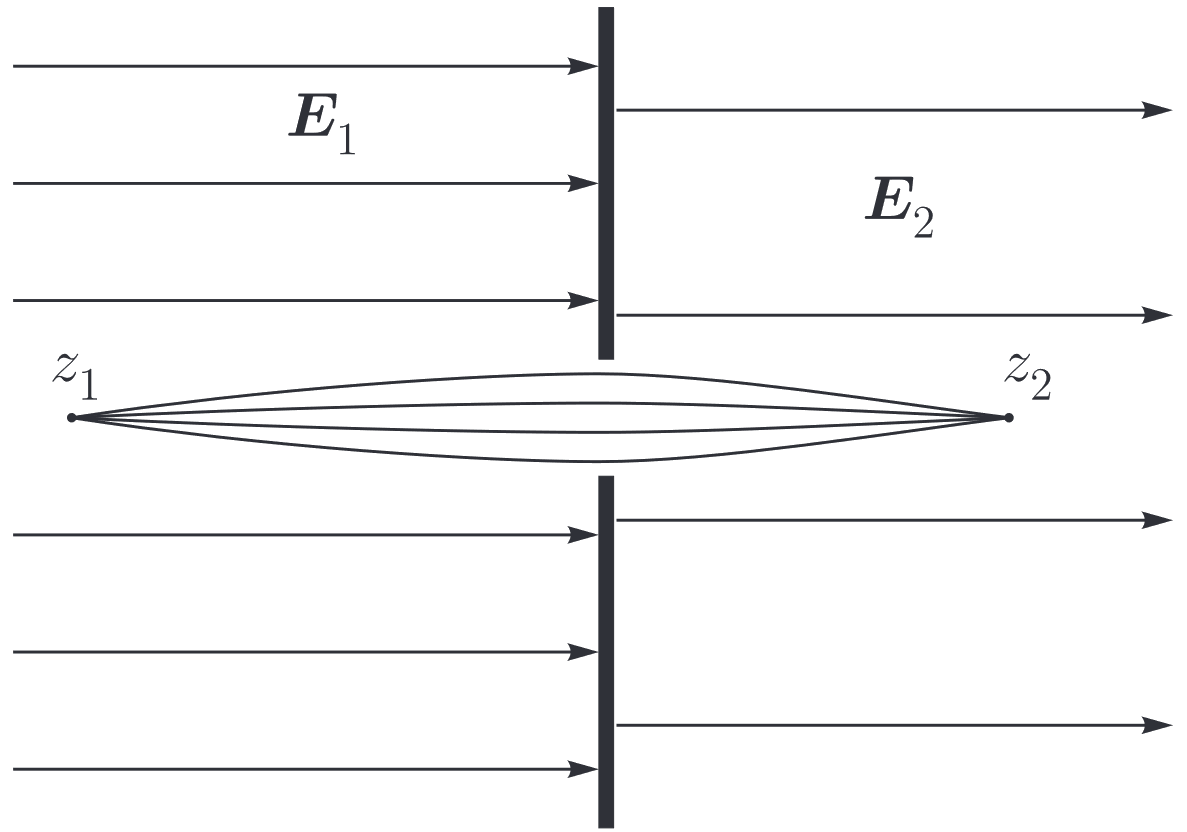
\includegraphics[width=0.5\textwidth]{S3 Figures/S3-74.png}
\end{center}
\end{solution}

\hypertarget{P75}{}
\begin{solution}{normal} % 75
a) Determine the electric field due to two non-conducting charged spheres of radius $R$ in their region of overlap. The volumetric charge densities of the spheres is $\pm \rho$ and the distance between the centres of the spheres is $d$.  b) Solve part a) if the two spheres are replaced by infinitely long parallel cylinders.
\begin{center}
    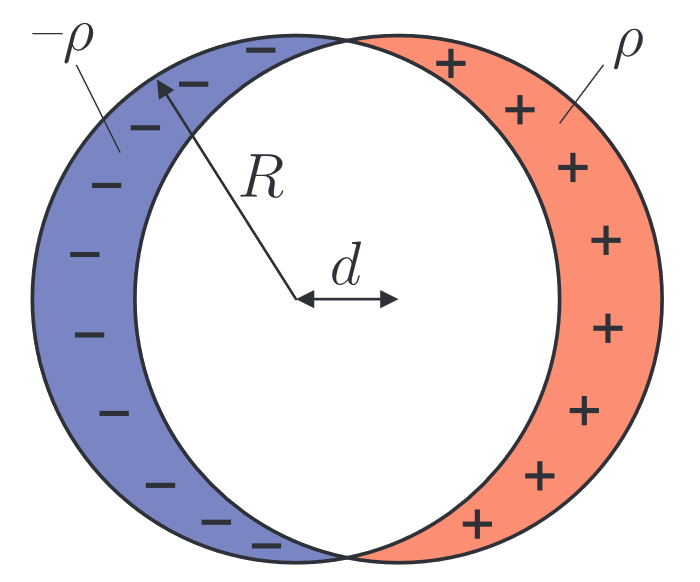
\includegraphics[width=0.4\textwidth]{S3 Figures/S3-75.png}
\end{center}
\end{solution}

\hypertarget{P76}{}
\begin{solution}{normal} % 76
Consider a uniformly charged sphere of charge density $\rho$. Inside this sphere is a spherical cavity located at a position $\textbf{\textit{r}}_0$ relative to the center of the sphere. Determine the electric field in the cavity.
\end{solution}

\hypertarget{P77}{}
\begin{solution}{normal} % 77
Show that the force acting between two spheres with uniform charge distribution is the same as the force between two point charges (i.e. $Q_1Q_2/(4\pi\varepsilon_0r^2)$), where $Q_1$ and $Q_2$ are the total charges on the spheres and $r$ is the distance between their centers.
\end{solution}

\hypertarget{P78}{}
\begin{solution}{normal} % 78
Determine the force between a uniformly charged infinitely long cylinder and a uniformly charged sphere. The linear charge density of the cylinder is $\lambda$, the total charge found on the sphere is $Q$ and $r$ is the distance from the centre of the sphere to the axis of the cylinder.
\end{solution}

\hypertarget{P79}{}
\begin{solution}{normal} % 79
Find the electrostatic pressure acting on the surface of a uniformly charged sphere if the surface charge density of the sphere is $\sigma$.
\end{solution}

\hypertarget{P80}{}
\begin{solution}{normal} % 80
Find the force exerted by one hemisphere of a non-conducting uniformly charged sphere having charge $Q$ and radius $R$ on the other hemisphere. \textit{Note:} This problem is also in Griffiths.
\end{solution}

\hypertarget{P81}{}
\begin{solution}{normal} % 81
Determine the electric field at a distance $r$ along the central axis of a dipole.
\end{solution}

\hypertarget{P82}{}
\begin{solution}{normal} % 82
Prove expression 4 for an electric dipole. \textit{Note:} Use the results of the previous problem to treat an arbitrarily oriented dipole as a superposition of two perpendicular dipoles. Essentially, this means adding additional fictitious charges $\pm q$ to a suitable points in space.
\begin{center}
    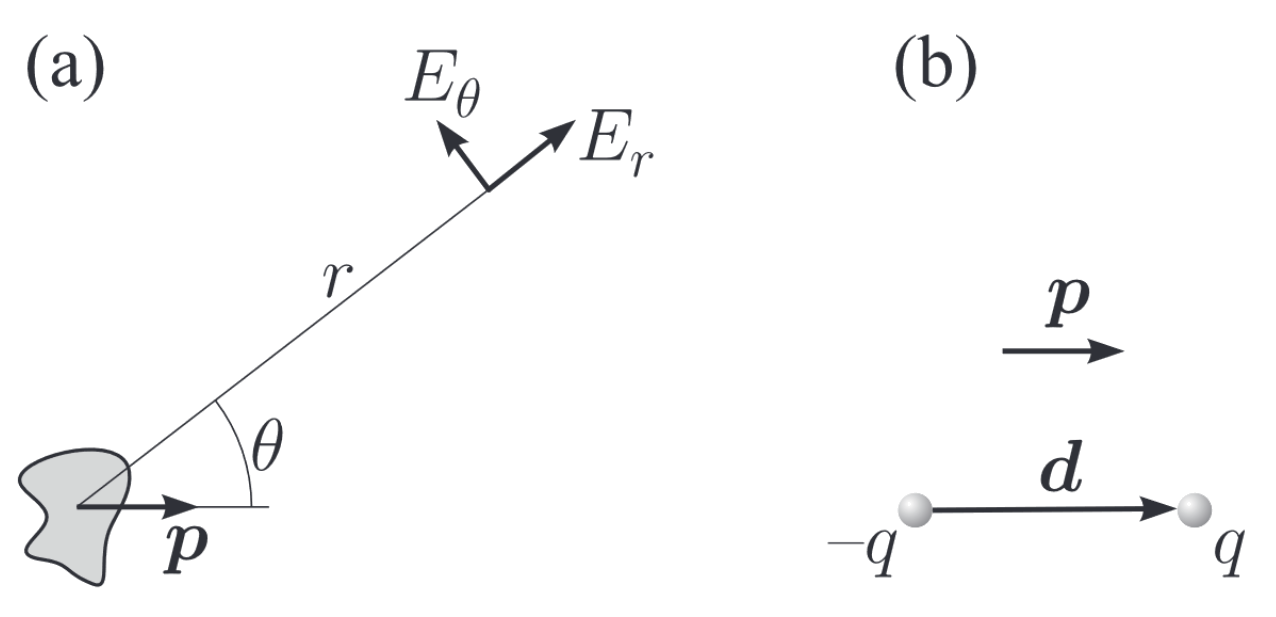
\includegraphics[width=0.5\textwidth]{S3 Figures/S3-82.png}
\end{center}
\blfootnote{Expression 4 (also see the figure above) gives $$E_r=\dfrac{2p\cos\theta}{4\pi\varepsilon_0r^3},\;\;\;E_\theta=\dfrac{p\sin\theta}{4\pi\varepsilon_0r^3}$$ where the quantity $\textbf{\textit{p}}=\sum q_i\textbf{\textit{r}}_i$ is known as the dipole moment of a system of charges}
\end{solution}

\hypertarget{P83}{}
\begin{solution}{normal} % 83
A parallel plate capacitor located in a vacuum is formed with two metal plates of area $S$. The capacitor is then charged to a voltage $U$. Determine the strength of the electric field in the plane of the plates at a distance $r$ from the plates, where $r$ is much larger than the dimensions of the plates.
\end{solution}

\hypertarget{P84}{}
\begin{solution}{normal} % 84
Find the torque acting on an electric dipole $\textbf{\textit{p}}$ when it is placed in an external electric field $\textbf{\textit{E}}$.
\end{solution}

\hypertarget{P85}{}
\begin{solution}{normal} % 85
Calculate the potential energy of an electric dipole $\textbf{\textit{p}}$ in an electric field $\textbf{\textit{E}}$.
\end{solution}

\hypertarget{P86}{}
\begin{solution}{normal} % 86
Determine the force acting between an electric dipole $\textbf{\textit{p}}$ and a point charge $q$ if they are separated by a distance $r$ and the vector $\textbf{\textit{p}}$ is directed towards the point charge. \textit{Note:} Here, a similar approach to that in P81 can be used. It is also possible to use a virtual shift approach like the one in P85. This problem gives an intermediate result for the more general formula $F_x=\textbf{\textit{p}}(\partial\textbf{\textit{E}}/\partial x)$.
\end{solution}

\hypertarget{P87}{}
\begin{solution}{normal} % 87
Determine the force between two dipoles $\textbf{\textit{p}}_1$ and $\textbf{\textit{p}}_2$ if the distance between the dipoles is $r$.
\end{solution}

\hypertarget{P88}{}
\begin{solution}{normal} % 88
Estimate the frequency of oscillation of a polar molecule in an electric field of $E=30\;\text{kV}/\text{m}$. We can model the molecule as a rigid dumbbell-shaped structure with length $l\sim 0.1\;\text{nm}$ and mass $m\sim 10^{-26}\;\text{kg}$. The magnitude of the charges $\pm q$ on the atoms are $1.6\times10^{-19}\;\text{C}$.
\end{solution}

\hypertarget{P89}{}
\begin{solution}{normal} % 89
The space $0<x<d$ has uniform charge density $\rho$ ($\rho>0$), and the space $-d<x<0$ has uniform charge density $-\rho$. There is no charge in the regions $-\infty<x<-d$ and $d<x<\infty$. In the region $x>d$, an electron with mass $m$ and charge $-e$ moves with its velocity vector pointed directly towards the charged space. What is the minimum initial velocity that the electron must have if it is able to pass through the charged space?
\end{solution}

\hypertarget{P90}{}
\begin{solution}{normal} % 90
Is it possible to generate an electric field with field lines as shown in the diagram below?
\begin{center}
    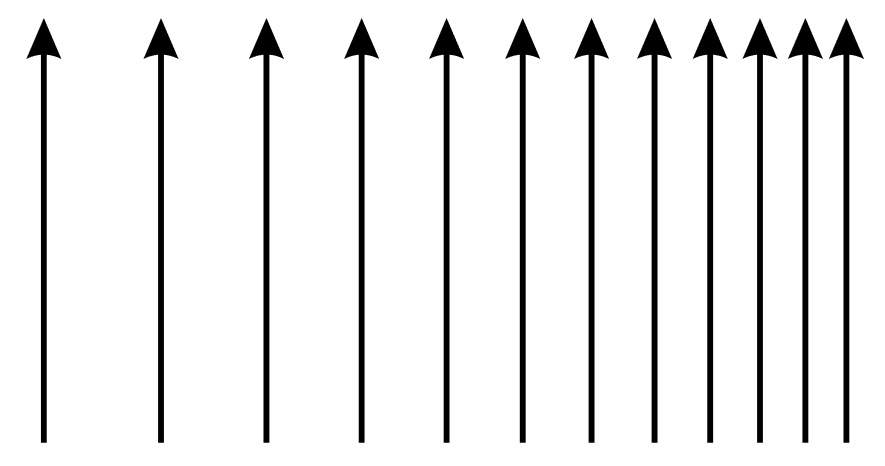
\includegraphics[width=0.5\textwidth]{S3 Figures/S3-90.png}
\end{center}
\end{solution}

\hypertarget{P91}{}
\begin{solution}{normal} % 91
Show that the potential inside a uniformly charged sphere is constant and equal to the potential of the sphere itself.
\end{solution}

\hypertarget{P92}{}
\begin{solution}{normal} % 92
a) Show that the capacitance of a parallel plate capacitor (in a vacuum) is given by the formula $\varepsilon_0 S/d$, where $S$ is the area of of the plates and $d$ is their distance of separation. b) Assuming that the electric field between the plates is $E$, show that the energy density of the capacitor is $\varepsilon_0 E^2/2$.
\end{solution}

\hypertarget{P93}{}
\begin{solution}{normal} % 93
$N$ identical droplets of mercury are charged to the same potential  $\varphi_0$. Determine the potential of a large drop of mercury when the $N$ smaller droplets coalesce (assume all the droplets are spherical).
\end{solution}

\hypertarget{P94}{}
\begin{solution}{normal} % 94
Show that the electric potential due to a dipole $\textbf{\textit{p}}$ can be expressed as $\varphi(r)=\textbf{\textit{p}}\hat{\textbf{\textit{r}}}/(4\pi\varepsilon_0r^2)$.
\end{solution}

\hypertarget{P95}{}
\begin{solution}{normal} % 95
A capacitor is formed from two concentric metal spheres, and the space between them is filled with air. If the radius of the outer sphere is $0.5\;\text{m}$ and if the air breaks down under an electric field of $30\;\text{kV}/\text{cm}$, what must the radius of the inner sphere be in order to create the highest possible potential difference? Also calculate that potential difference.
\end{solution}

\hypertarget{P96}{}
\begin{solution}{normal} % 96
Determine the strength of the electric field a distance $x$ along the axis of a ring of radius $R$ with charge $Q$ distributed evenly over its surface.
\end{solution}

\hypertarget{P97}{}
\begin{solution}{normal} % 97
Determine the radius of an electron assuming that the mass of an electron ($m_e=9.1\times10^{-31}\;\text{kg}$) is due to the electrostatic energy of its charge ($\Pi=mc^2$). In our simple model, you may assume that the charge of the electron ($e=-1.6\times10^{-19}\;\text{C}$) is evenly distributed over its "surface". 
\end{solution}

\hypertarget{P98}{}
\begin{solution}{normal} % 98
Two metal spheres with radii $R_1$ and $R_2$ are spaced a very far distance apart. If both spheres initially have charge $q$, what will the charges on the spheres be once they are connected by a wire?
\end{solution}

\hypertarget{P99}{}
\begin{solution}{normal} % 99
A point charge $q$ is placed a distance $h$ above an infinite planar conductor. Determine the surface charge density $\sigma$ induced on the surface of the conductor.
\end{solution}

\hypertarget{P100}{}
\begin{solution}{normal} % 100
A metal sphere with radius $r$ is given charge $q$. The sphere is connected to the ground with a long wire of resistance $R$. Determine the initial current through the wire.
\end{solution}

\hypertarget{P101}{}
\begin{solution}{normal} % 101
A metal sphere of radius $r$ is located inside a larger metal sphere of radius $R$. The two spheres are concentric, and the smaller sphere is grounded by a long wire (that passes through a small opening on the surface of the larger sphere). The larger sphere has no contact with the other sphere or the grounding wire. a) The outer sphere is given a charge $Q$. What charge is induced on the smaller sphere as a result? b) Determine the capacitance of the spheres.
\end{solution}

\hypertarget{P102}{}
\begin{solution}{normal} % 102
A point charge $q$ is located a distance $r$ from the center of a metal sphere of radius $R$. What is the potential of the sphere?
\end{solution}

\hypertarget{P103}{}
\begin{solution}{normal} % 103
A point charge $q$ is at a distance $h$ above the surface of a conductor in the shape of an infinite plane. What is the force acting on this point charge?
\end{solution}

\hypertarget{P104}{}
\begin{solution}{normal} % 104
A metal sphere of radius $R$ is placed in a homogeneous electric field $\textbf{\textit{E}}_0$. Determine the charge density on the surface of the sphere and the electric field in the space around the sphere. \textit{Note:} The field outside the sphere due to the surface charge density is similar to the field caused by a dipole placed at the center of the sphere (see P94).
\end{solution}

\hypertarget{P105}{}
\begin{solution}{normal} % 105 ? can't translate note
A metal cylinder of radius $R$ is placed in a homogeneous electric field $\textbf{\textit{E}}_0$ with its axis perpendicular to the field. Determine the charge density induced on the surface of the cylinder and the electric field in the space around the cylinder.
\end{solution}

\hypertarget{P106}{}
\begin{solution}{normal} % 106
A charge $q$ is located at a distance $h$ from the center of a grounded metal sphere of radius $R$. Find the force acting on the charge.
\end{solution}

\hypertarget{P107}{}
\begin{solution}{normal} % 107
Solve the previous problem if the sphere is not grounded. \textit{Tip:} The solution to P106 only needs to be slightly improved.
\end{solution}

\hypertarget{P108}{}
\begin{solution}{normal} % 108
The two plates in a parallel plate capacitor each have area $S$ and are separated by a distance $d$. Both plates are grounded. A point charge $q$ is placed between the two plates at a distance $x$ from the first plate. How much charge accumulates on each plate?
\end{solution}

\hypertarget{P109}{}
\begin{solution}{normal} % 109 ? unsure about translation
A dielectric with dielectric constant $\kappa$ is inserted between the plates of a parallel plate capacitor with area $S$ and separation $d$. a) Find the capacitance of the capacitor; b) Find the force acting between the plates of the capacitor when a potential difference of $U$ is applied across the plates 
\end{solution}

\hypertarget{P110}{}
\begin{solution}{normal} % 110
A parallel plate capacitor is immersed in a non-conductive fluid with dielectric constant $\kappa$. Determine the force between the plates if the area of the plates is $S$, their separation is $d$, and the charges on them are $\pm Q$.
\end{solution}

\hypertarget{P111}{}
\begin{solution}{normal} % 111
A dielectric slab with uniform thickness and dielectric constant $\kappa$ is placed in a homogeneous electric field $\textbf{\textit{E}}_0$, with which the plate forms an angle $\theta$. Determine the electric field inside the plate and the charge density on the surface of the plate.
\end{solution}

\hypertarget{P112}{}
\begin{solution}{normal} % 112
An infinitely long dielectric cylinder with dielectric constant $\kappa$ is placed in a homogeneous electric field $\textbf{\textit{E}}_0$. Determine the electric field inside the cylinder if the axis of the cylinder: a) is parallel to $\textbf{\textit{E}}_0$; b) lies across $\textbf{\textit{E}}_0$.
\end{solution}

\hypertarget{P113}{}
\begin{solution}{normal} % 113
Consider a dielectric sphere of radius $R$ and dielectric constant $\kappa$. Determine the field inside the sphere and the surface charge density on the surface of the sphere.
\end{solution}

\hypertarget{P114}{}
\begin{solution}{normal} % 114
A point charge $q$ is kept at a distance $h$ from the line separating two infinite dielectric planes. The dielectric constants of the planes are $\kappa_1$ and $\kappa_2$ respectively. Find the electric field in each dielectric.
\end{solution}

\hypertarget{P115}{}
\begin{solution}{normal} % 115
Determine the force acting on a dielectric sphere of radius $R$ and dielectric constant $\kappa$ in an inhomogeneous electric field $\textbf{\textit{E}}(\textbf{\textit{r}})$. \textit{Note:} See problem 113 and problem 86.
\end{solution}